\section{Design Requirements \& Hardware Implementation} \label{sec:hardware}\label{sec:design_requirements}

\subsection{Hardware}
The apparatus consists of the housing, which has been installed in CRH (Fig.~\ref{fig:CALIS_photos}, left) and the deployment device which can be lowered into the LSV (Fig.~\ref{fig:CALIS_photos}, right). The deployment device is attached to the housing through two stainless steel cables that are wound up on cable spools (Fig.~\ref{fig:CALISMechanism}).

\subsubsection{Deployment \& Articulation}\label{sec:DeploymentArticulation}
The center of the \lsv\ is about 6 m below the gate valve inside CRH
%=6145=70+120+400+3455+20+251+1372+457 from http://darkside-docdb.fnal.gov:8080/cgi-bin/RetrieveFile?docid=858&filename=NoFlyZone-DS50_vers02.pdf&version=14
 and the $6''$ wide organ pipes are vertical, yet about 80 cm off center in the XY plane as shown in Fig.~\ref{fig:CALIS_photos}. For \tpc\ calibration the radioactive source has to be positioned in immediate contact with the cryostat, in order to minimize rate losses through absorption in particular for low energy sources such as $^{57}$Co (122 keV). This is made possible by enabling the deployment device to articulate an arm, at whose end the radioactive source is thereby brought close the cryostat. 

\begin{figure}[htbp]
 \centering
 %\subfigure{ 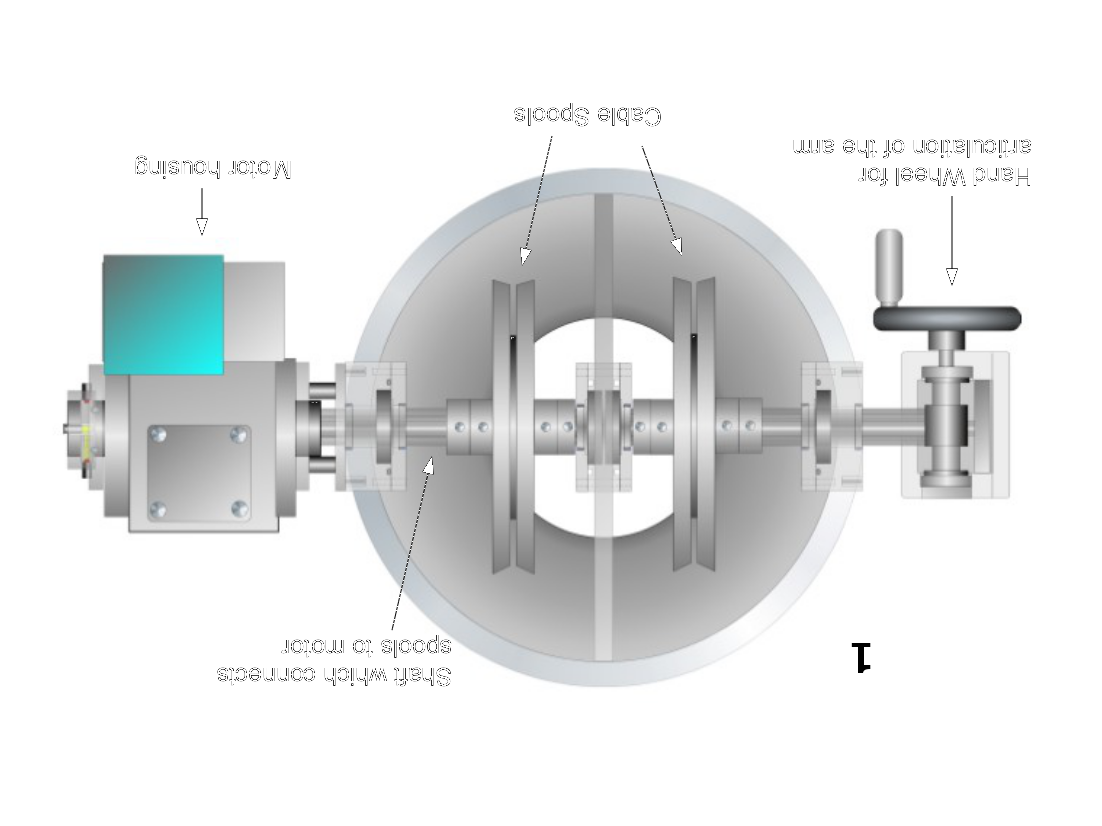
\includegraphics[width=0.7\textwidth]{Figures/gearDrawing}}
 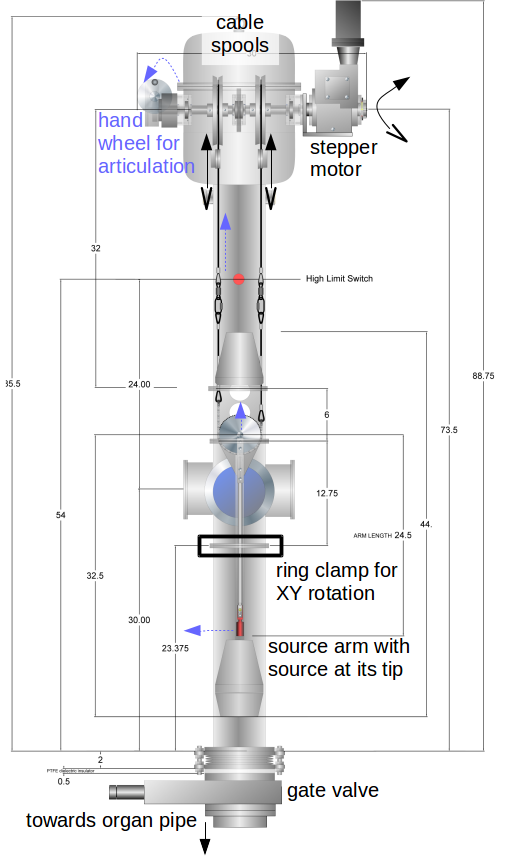
\includegraphics[width=0.72\textwidth]{Figures/CALISDimensions.png}
 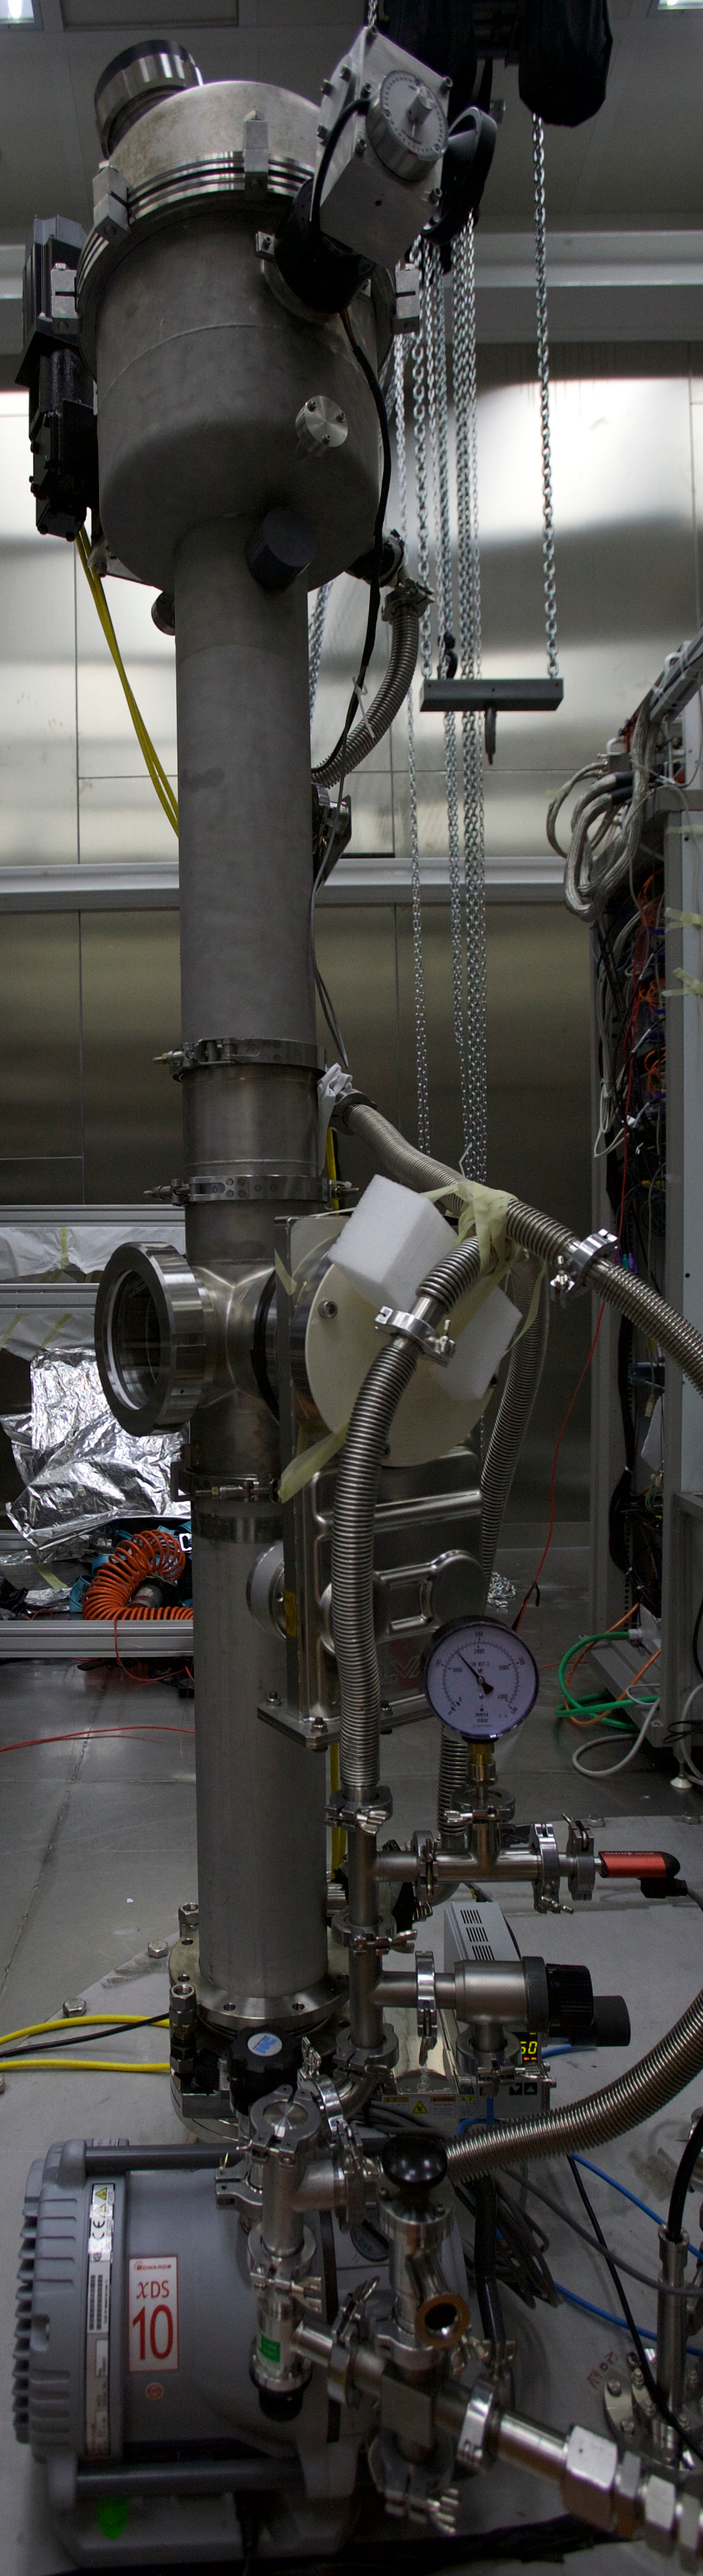
\includegraphics[width=0.27\textwidth]{Figures/CALIS_overview_IMG_3763.jpg}
 \caption{%\textit{top}:Looking down on the top of CALIS III and inside the upper assembly: the components and drive mechanism are shown. The hand wheel is on the left connected to one of the spools only. The next parts going from left to right are the two cable spools and then the sealed motor housing.
Mechanical drawing of CALIS showing the housing and the deployment device. Dimensions are in inches. (The total height of 88.75 inches corresponds to 225.425 cm.) The two modes of operation are illustrated: In order to move the deployment device downinto the LSV or back up the stepper motor moves both cable spools simultaneously. \textcolor{blue}{In order to articulate, the articulation wheel is rotated manually, which affects only the left spool, thereby shortening the left cable wrt.~to the right cable thereby articulating the arm and lifting the pivot center.} The amount of lifting and the amount of rotations until a horizontal articulation is reached has been calibrated prior to installation in CRH (Sec.~\ref{sec:Testing:LNGS})\label{fig:CALISDimensions}\label{fig:CALISMechanism}\label{fig:gearDrawing}
}
\end{figure}

In order to send the deployment device into the LSV, both cables are unwound simultaneously. The stepper motor moves both cable spools concurrently and an absolute encoder monitors the current position of the deployment device. The stepper motor is controlled via a simple graphical LabVIEW interface, run on a dedicated laptop, in which the current z-position is shown and a target z-position can be provided by the operator. Z-positions are given in motor step counts, an arbitrary unit which has been calibrated outside CRH in meters and relative to the TPC using calibration data.

Articulation of the arm is done manually via the articulation wheel (Fig.~\ref{fig:CALISMechanism}). This affects only the cable spool close to the articulation wheel, the left one in Fig.~\ref{fig:CALISMechanism}, thereby shortening the left cable wrt.~to the right cable and engaging the gear through a chain (Fig.~\ref{fig:sourceArmRotation}). As a result the arm is articulated and the pivot center is lifted. The degrees corresponding to a horizontal articulation has been calibrated prior to installation in CRH (Sec.~\ref{sec:Testing:LNGS}).

%The deployment and articulation mechanism involving two steel cables

Articulation and a movement in z-direction are mutually exclusive since the articulation of the arm leads to more wound up cable on the spool close to the articulation wheel wrt.~the other. If then in deployment mode both spools would be rotated simultaneously with the same angular speed, the cable close to the articulation wheel would wind up faster than the other, which would lead to a build up of difference in cable length and the deployment device would only be hanging on one cable. In order to avoid an imbalanced z-movement the arm has to be dearticulated before a change in z-position can be initiated. This is enforced by an electric switch preventing z-movement, which is disengaged only when the arm is fully dearticulated. 

\begin{figure}[htbp]
 \centering
\begin{minipage}[b]{0.48\textwidth}
\centering
  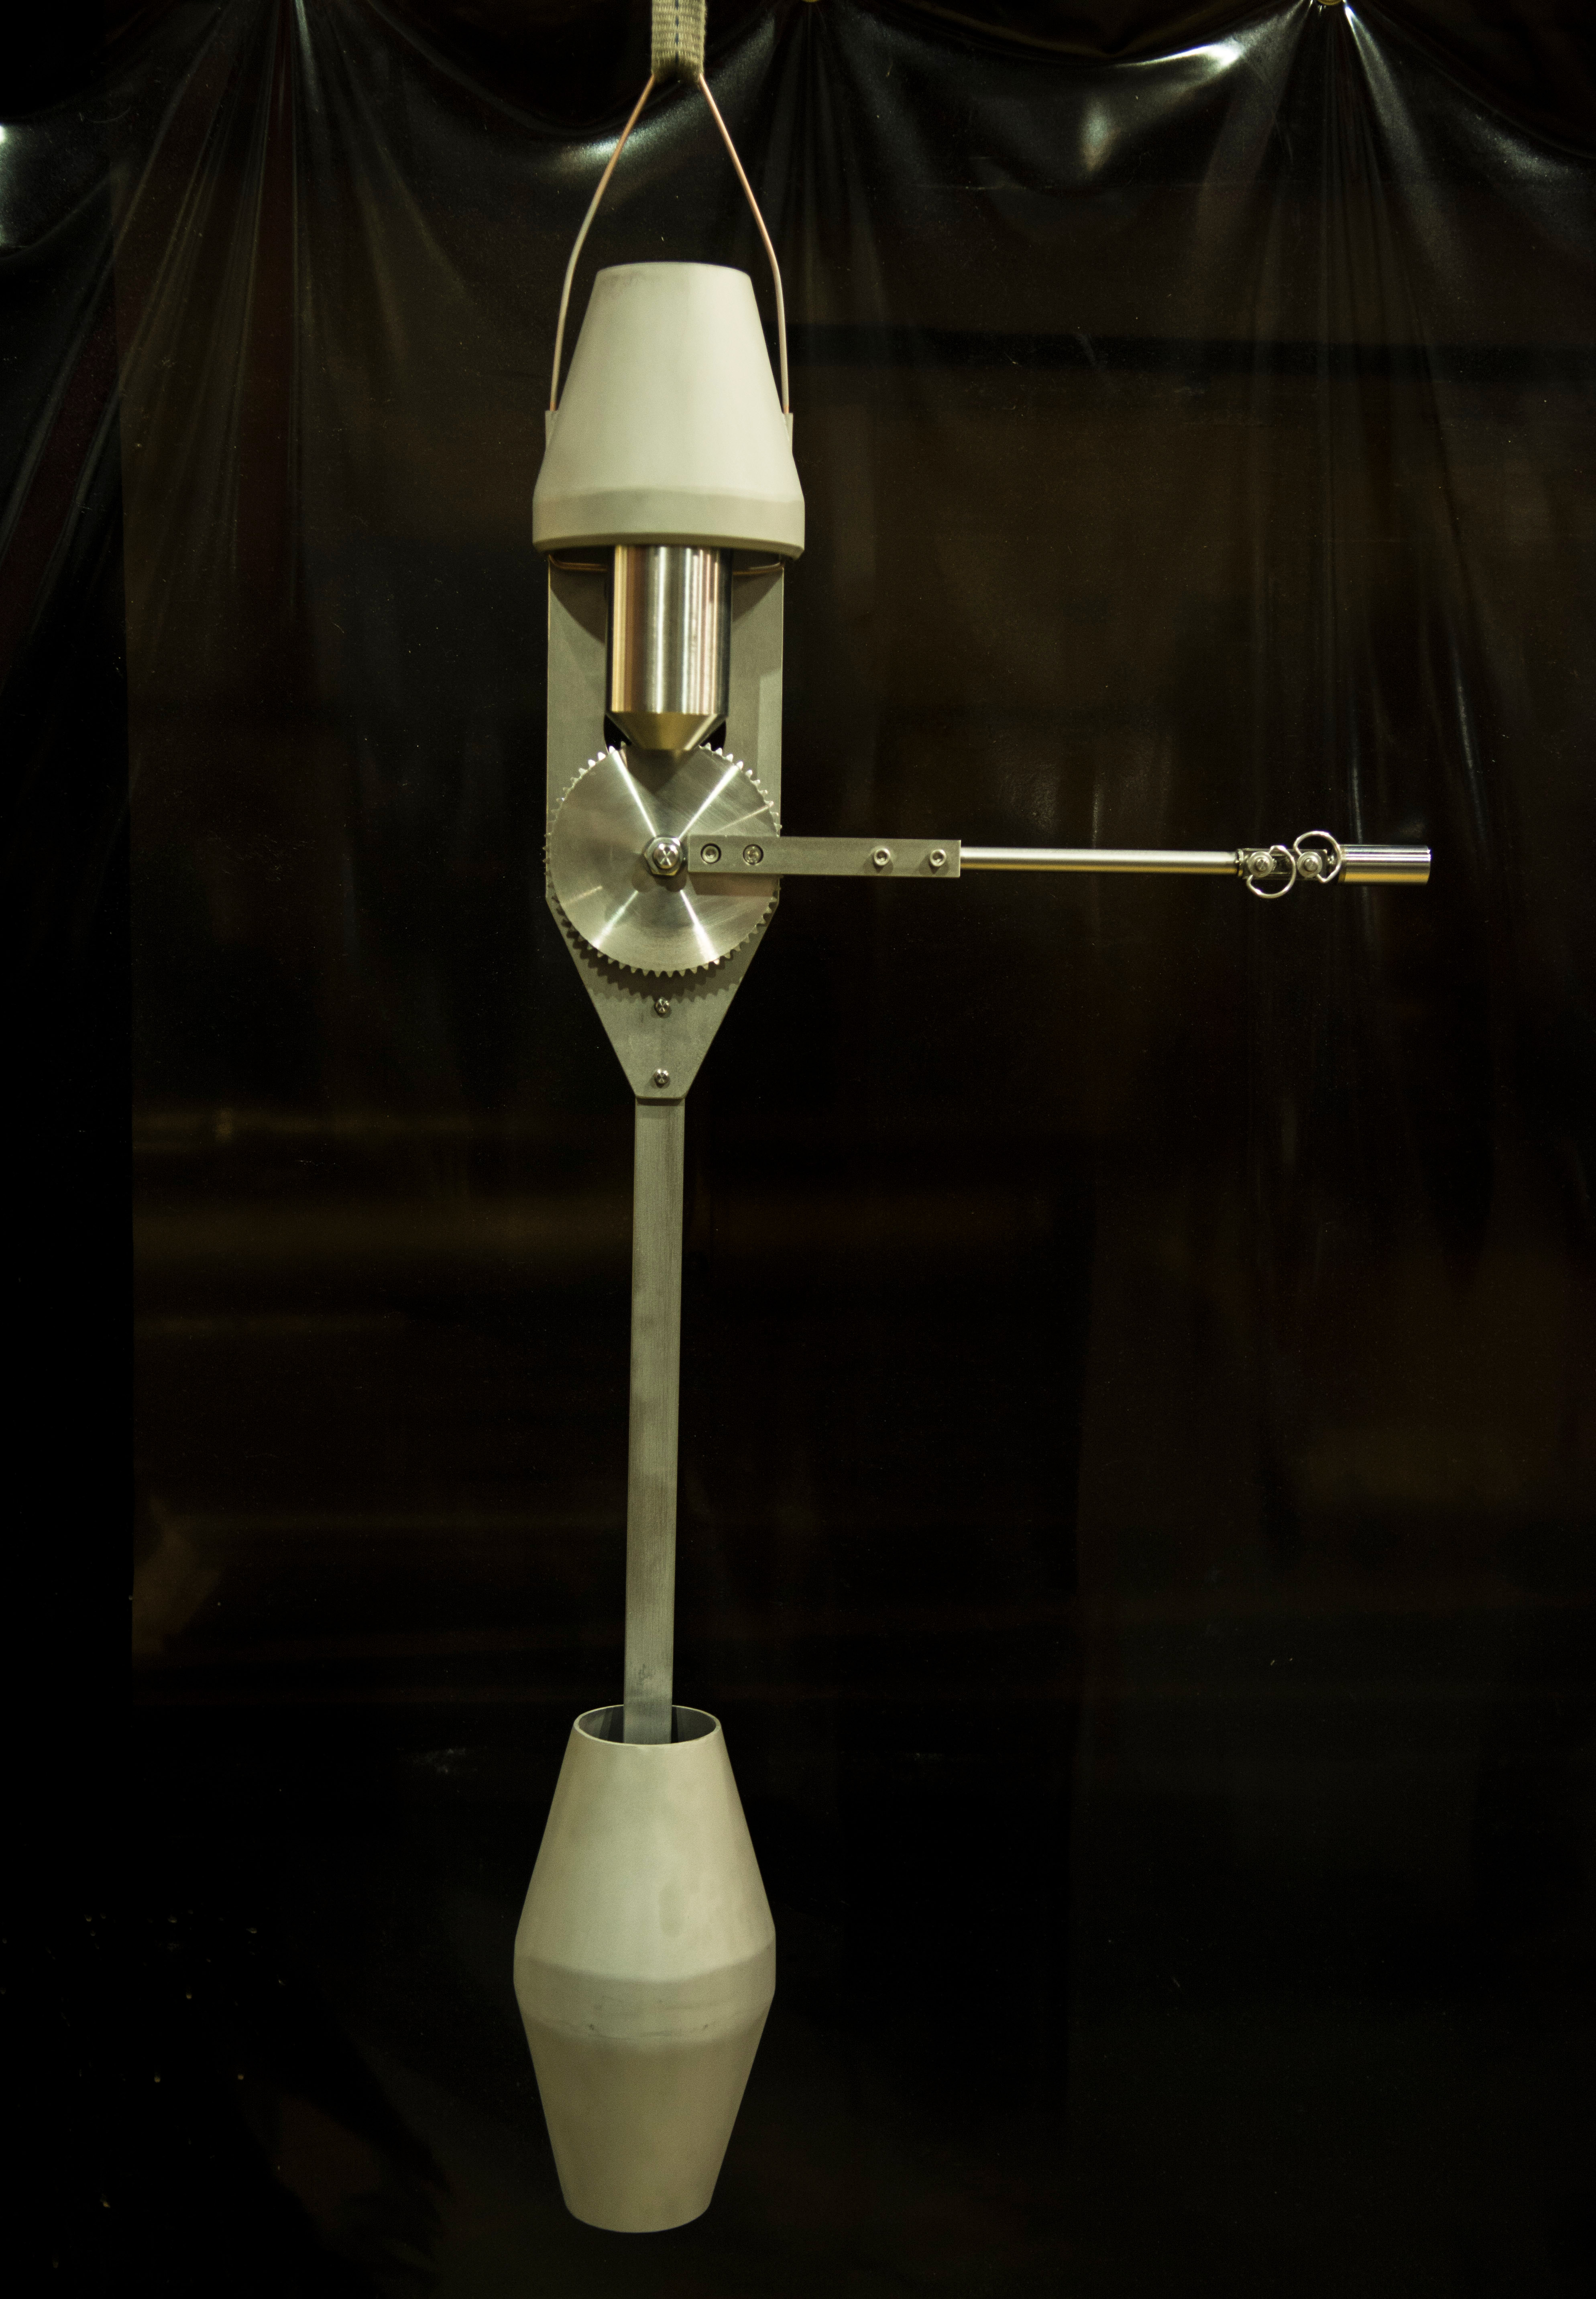
\includegraphics[width=\textwidth]{Figures/SourcePod2_mirrored.jpg}
\end{minipage}
\begin{minipage}[b]{0.48\textwidth}
\centering
  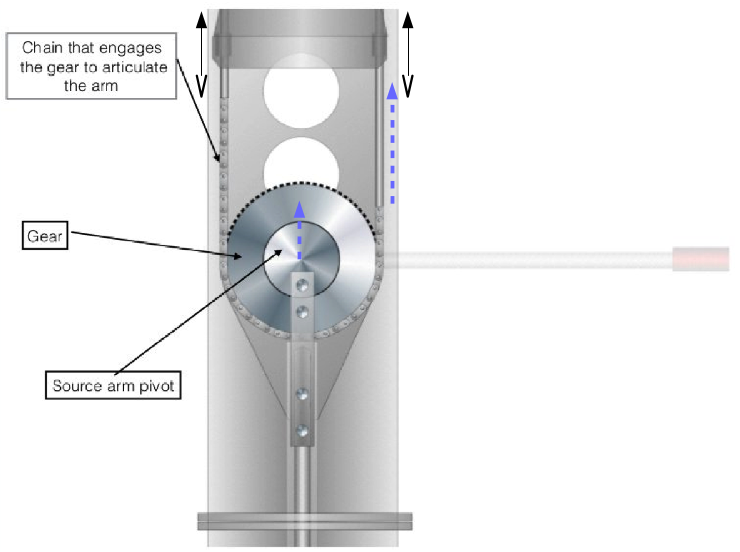
\includegraphics[width=\textwidth]{Figures/sourceArmArticulation.png}
  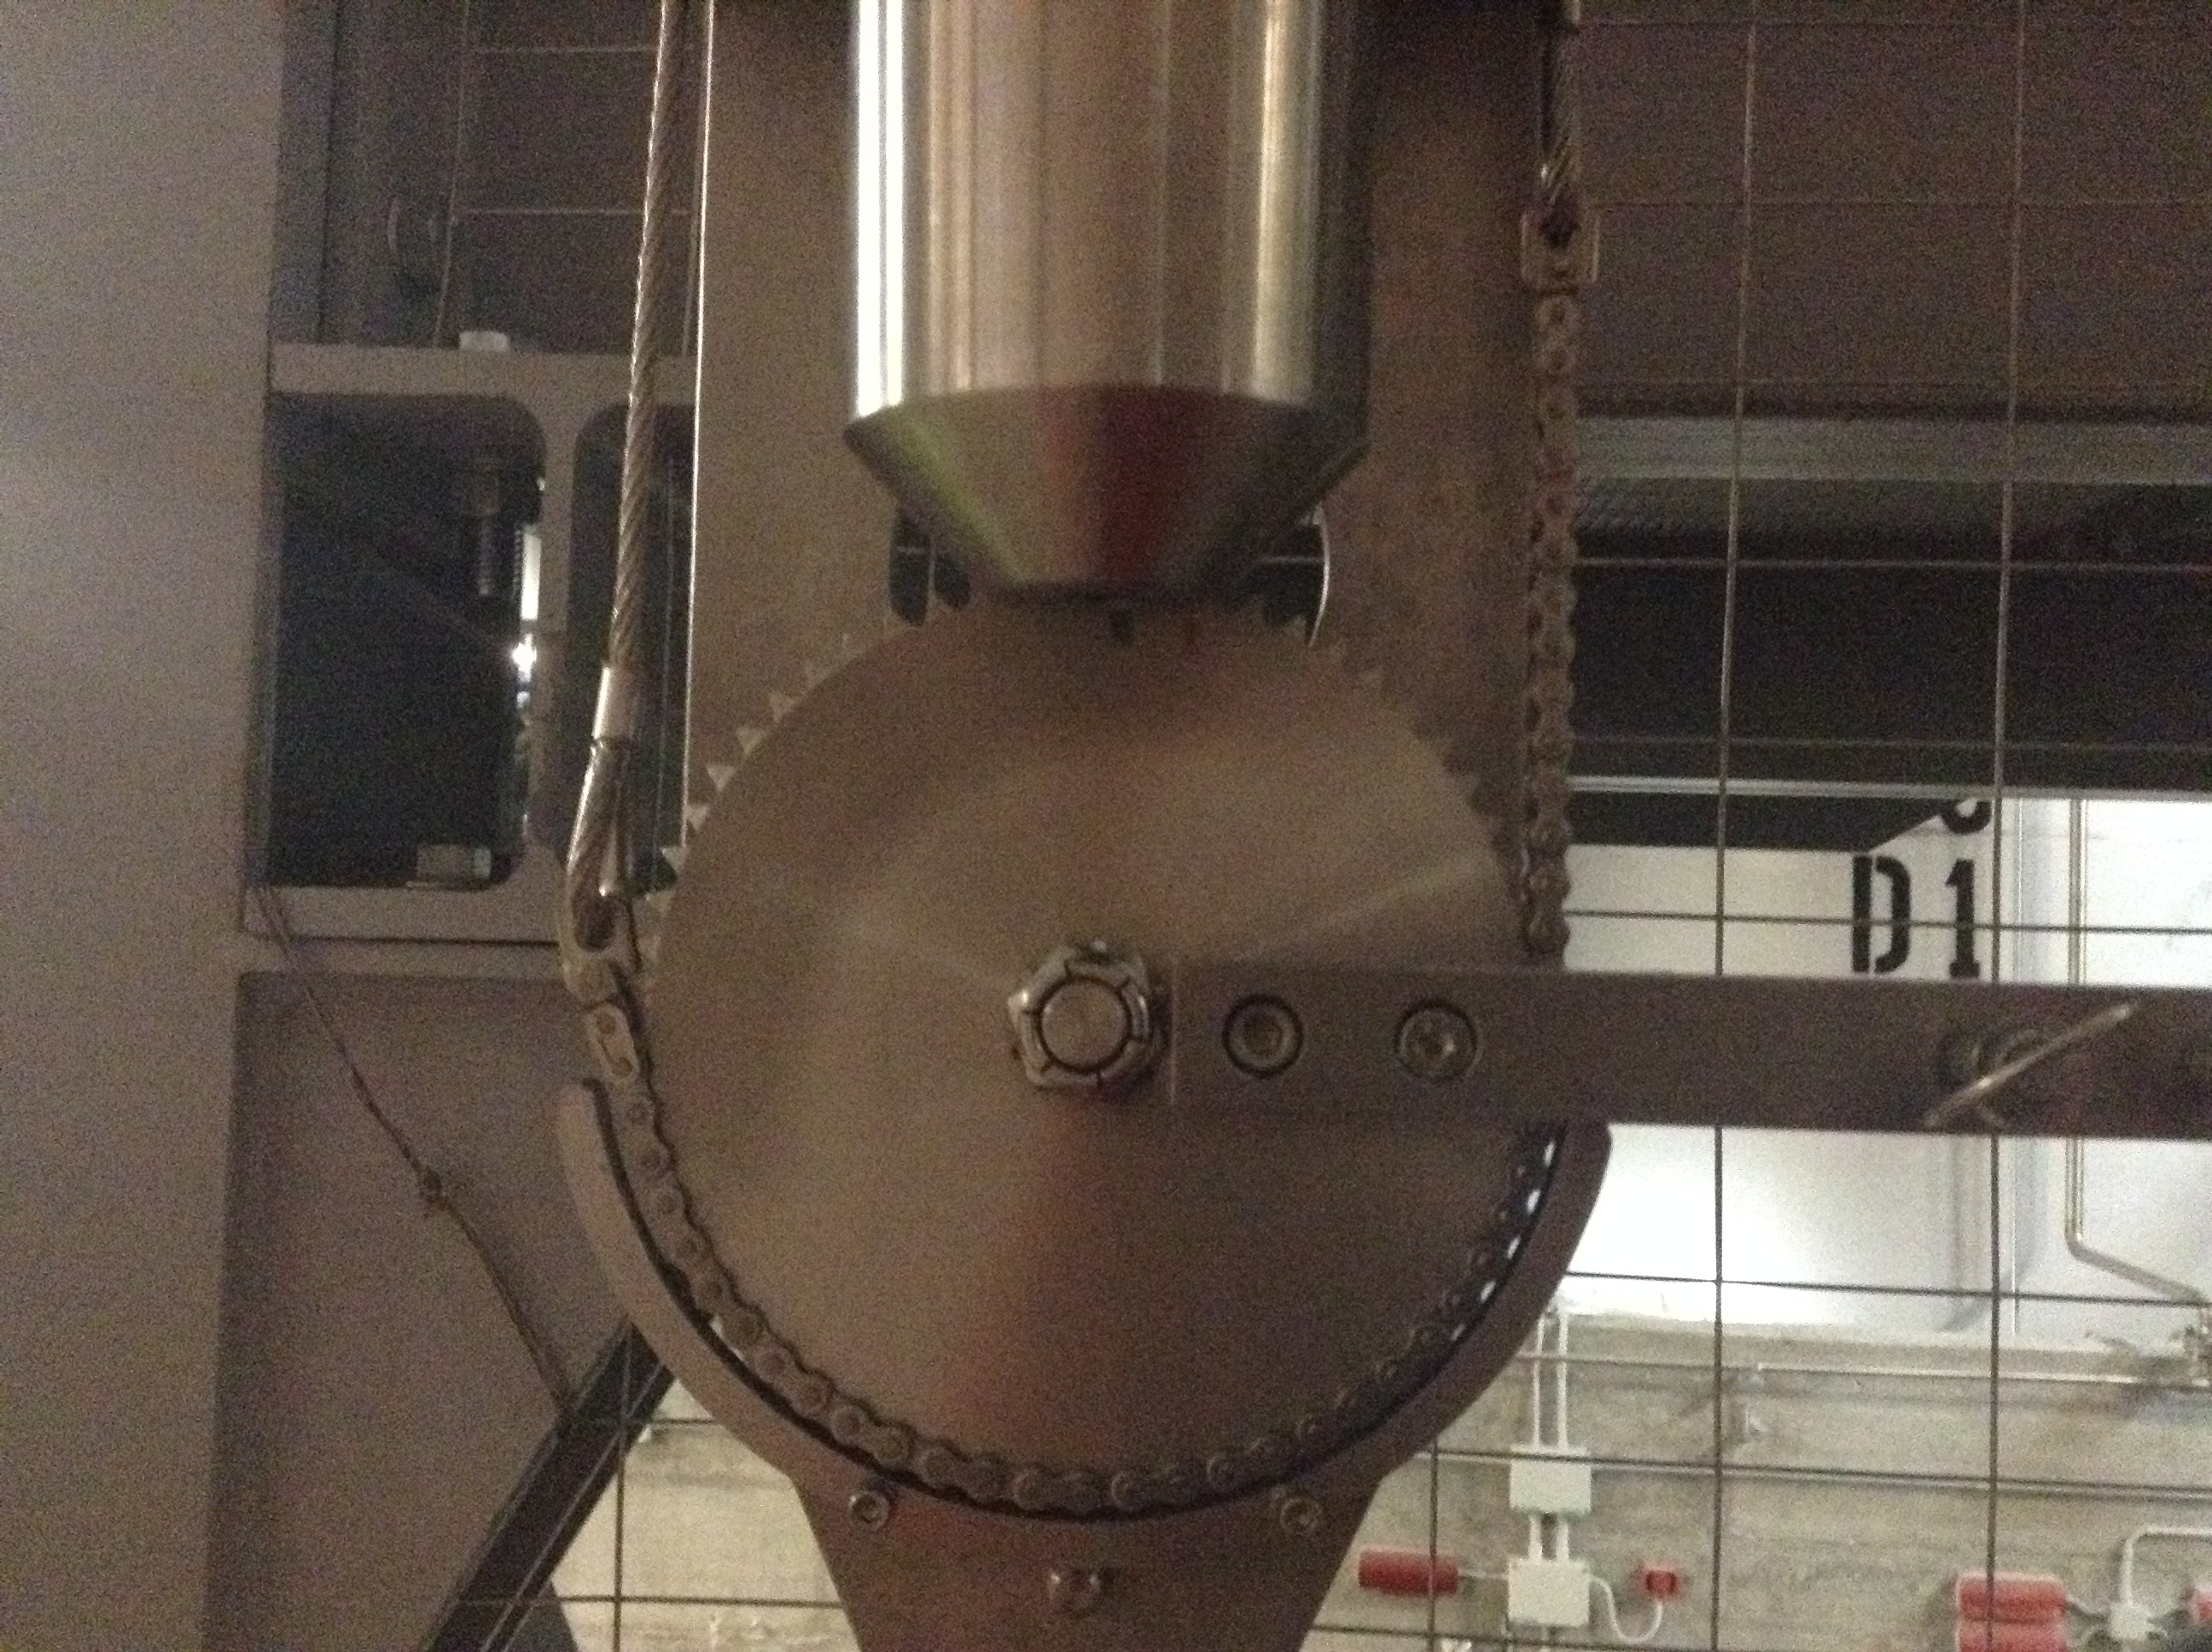
\includegraphics[width=0.8\textwidth]{Figures/IMG_2457.JPG}
\end{minipage}
  \caption{Technical drawing showing the articulation mechanism using a chain that engages the gear to transfer the rotation of the articulation wheel (Fig.~\ref{fig:CALISMechanism}) into a rotation of the source arm. The chain has a guard rail, not shown in the drawing, that ensures that the chain can never come off the gear.}
  \label{fig:sourceArmRotation}
\end{figure} 

\subsubsection{Housing \& Scintillator}

Besides providing mechanical support for the deployment device, the housing is the important interface between CRH and the LSV, through which sources are exchanged, while protecting the liquid scintillator and avoiding human contact with the liquid scintillator. The liquid scintillator, which is a mixture of PC and TMB\footnote{As discussed in Sec.~\ref{sec:CalibCampaigns} the concentration of TMB has varied during the campaigns.} with the wavelength shifter PPO\cite{DS50:firstPaper}, may not get exposed to oxygen or water as is present in normal clean room air and also contamination with $^{222}$Rn and its daughters has to be avoided. Vacuum and nitrogen pressurization systems have been developed \ref{sec:N2_pressure_system}.

On the other hand TMB vapors and residues could form ...

\textit{ToDo: more precise on risks of contact of TMB with air/ water. What are the dangers compared to a PC only scintillator?}

The housing thereby has the same role as glove boxes in calibration devices of other experiments (see e.g.~\cite{KamLAND:Calib,Borexino:Calib}).

\subsection{Design Requirements}
The design of CALIS is shaped by the following requirements, thereby following the design principle of ``form follows function'': 
\begin{itemize}
\item to allow source exchanges and safely deploy them at various positions inside the LSV, 
\item protecting the scintillator from oxygen and water at any time, in particular during deployments and being able to articulate a source arm in order to bring the source next to the cryostat. Also protection and safety mechanisms that avoid exposure of personal to scintillators are in place.
\item To complement studies of nuclear recoils with neutron sources ($^{241}$Am$^{9}$Be and $^{241}$Am$^{13}$C), it is planned to deploy a neutron gun inside a dedicated deployment device currently under development (Section \ref{sec:Outlook}).
\item All materials that come in contact with the scintillator veto are made of stainless steel and teflon except for the sealing o-rings which are made out of viton.  All three materials (stainless steel, teflon, and viton) are certified materials for contact with TMB and PC.
\item Before assembly in CRH, each component of CALIS, the ones introduced into the scintillator as well as those in the clean room CRH, have been subjected to the official cleaning procedure \cite{DS50:cleaning}.
\end{itemize}

This results in further hardware design choices and requirements that are discussed below.